\documentclass[9pt]{article}
\usepackage[a4paper,margin=0.62in]{geometry}
\usepackage[T1]{fontenc}
\usepackage{lmodern}
\usepackage{microtype}
\usepackage{amsmath,amssymb}
\usepackage{booktabs}
\usepackage{longtable}
\usepackage{graphicx}
\usepackage{xcolor}
\usepackage{fancyhdr}
\usepackage{enumitem}
\usepackage{hyperref}
\usepackage{array}
\graphicspath{{../figures/}{figures/}}
\setlength{\parindent}{0pt}
\setlength{\parskip}{3pt}
\setlist{nosep,leftmargin=*}
\hypersetup{colorlinks=true,linkcolor=black,urlcolor=blue}
\pagestyle{fancy}
\fancyhf{}
\fancyhead[L]{TCCP: Trustworthy Customer Churn Prediction}
\fancyhead[R]{Technical Paper}
\fancyfoot[C]{\thepage}

\newcommand{\figpair}[4]{%
\begin{figure}[!ht]
\centering
\begin{minipage}[t]{0.48\textwidth}\centering\includegraphics[width=\linewidth]{#1}\caption{#2}\end{minipage}\hfill
\begin{minipage}[t]{0.48\textwidth}\centering\includegraphics[width=\linewidth]{#3}\caption{#4}\end{minipage}
\end{figure}}

\title{\vspace{-1.0em}\textbf{TCCP: Trustworthy Customer Churn Prediction\\for Retention-Budget Allocation}}
\author{Group 15}
\date{}

\begin{document}

\begin{titlepage}
\thispagestyle{empty}
\centering
\vspace*{1.0cm}
{\Large\textsc{Group 15 Technical Paper}\par}
\vspace{1.0cm}
{\LARGE\bfseries TCCP\par}
\vspace{0.2cm}
{\Large Trustworthy Customer Churn Prediction\par}
\vspace{0.2cm}
{\large From customer data to governed retention action\par}
\vspace{0.9cm}
\rule{0.84\textwidth}{0.8pt}\par
\vspace{0.65cm}
{\large A reproducible machine-learning, explainability, and MLOps system\par}
\vspace{0.9cm}
\includegraphics[width=0.82\textwidth]{model_metrics.png}\par
\vfill
{\large IBM Telco Customer Churn Dataset\par}
\vspace{0.2cm}
{\large MLflow \textbullet{} Model Registry \textbullet{} FastAPI \textbullet{} CI/CD\par}
\vspace{0.55cm}
{\large August 2026\par}
\end{titlepage}

\setcounter{page}{1}
\begin{center}
{\Large\bfseries TCCP: Trustworthy Customer Churn Prediction for Retention-Budget Allocation\par}
\vspace{0.15cm}{\large Group 15\par}
\end{center}

\begin{abstract}
Churn prediction becomes valuable only when it supports a safe and explainable decision. TCCP is an end-to-end system that turns the IBM Telco Customer Churn dataset into calibrated customer-risk estimates, interpretable drivers, and a ranked retention action list. The system cleans the source data, compares five classifiers, selects an RBF support-vector classifier (SVC) using validation PR-AUC, evaluates discrimination and calibration on a held-out test set, and converts risk into expected net value under a contact budget. The final model achieved test ROC-AUC $=0.846$, PR-AUC $=0.667$, and Brier score $=0.137$. The implementation also packages feature contracts, batch scoring, model registry stages, an API, and CI/CD controls so that a prediction can be traced from input data to production action.
\end{abstract}

\textbf{Keywords:} customer churn, trustworthy AI, probability calibration, SHAP, partial dependence, retention optimization, MLOps

\section*{1. TCCP problem statement}
Telecom churn is not only a classification problem. A business team must decide which customers to contact, what evidence supports that decision, and how many contacts the budget can afford. A model that maximizes accuracy while producing poorly calibrated probabilities can waste offers on low-risk customers or miss customers who need intervention.

TCCP defines the operational problem as follows. For a customer with feature vector $x$, estimate the probability of churn:
\begin{equation}
 p(x)=P(Y=1\mid X=x), \qquad Y\in\{0,1\},
\end{equation}
where $Y=1$ means that the customer churns. The system then ranks customers using expected intervention value:
\begin{equation}
 U(x)=p(x)\,r\,v-c,
\end{equation}
where $r$ is the assumed save rate, $v$ is customer value, and $c$ is contact cost. Under a finite budget, customers are selected from the highest-ranked risk until the contact limit is reached. This separation between prediction and action is central: model quality determines ranking, while business assumptions determine intervention.

\textbf{Research question.} Can a reproducible pipeline produce reliable churn probabilities, explain why risk changes, and allocate retention contacts transparently under a fixed budget?

\section*{2. Solution architecture}
TCCP follows a problem-to-solution chain:

\begin{center}
\begin{tabular}{>{\raggedright\arraybackslash}p{0.18\textwidth} >{\centering\arraybackslash}p{0.06\textwidth} >{\raggedright\arraybackslash}p{0.62\textwidth}}
\toprule
\textbf{Business problem} & & \textbf{TCCP solution}\\
\midrule
Messy customer records & $\rightarrow$ & Leakage-safe cleaning, numeric coercion, imputation, encoding, and a versioned 32-feature contract.\\
Risk scores are hard to compare & $\rightarrow$ & Five-model benchmark, validation PR-AUC selection, held-out evaluation, and calibration diagnostics.\\
Black-box scores are difficult to trust & $\rightarrow$ & SHAP global explanations, SHAP dependence plots, partial dependence, and permutation importance.\\
Retention budget is limited & $\rightarrow$ & Probability ranking, action tiers, and expected net value by contact budget.\\
Models drift or become untraceable & $\rightarrow$ & Serialized artifact, metadata, registry stages, batch scoring, API health checks, and CI/CD validation.\\
\bottomrule
\end{tabular}
\end{center}

The design principle is traceability. Every production score should be reproducible from the model version, feature schema, input record, and scoring code. The system therefore treats data quality, probability quality, explainability, and deployment governance as one product rather than separate notebooks.

\section*{3. Data understanding and preparation}
The raw IBM Telco Customer Churn file contains 7,043 customers. The cleaning stage strips column names, converts the whitespace-encoded \texttt{TotalCharges} field to numeric values, maps \texttt{Churn} from Yes/No to 1/0, removes \texttt{customerID} from model inputs, and separates target from predictors. Numeric fields are median-imputed and standardized; categorical fields are most-frequent-imputed and one-hot encoded inside a scikit-learn pipeline. Engineered variables include service count, tenure bins, charge interactions, charge-per-tenure, logarithmic charges, and a new-customer flag.

\begin{table}[!ht]
\centering\small
\begin{tabular}{ll}
\toprule
\textbf{Data contract item} & \textbf{Observed implementation}\\
\midrule
Source & IBM Telco Customer Churn dataset\\
Rows retained & 7,043 customers\\
Raw missing values & 11 whitespace values in \texttt{TotalCharges}\\
Cleaned feature count & 32 columns\\
Target & \texttt{Churn}: 1 = churn, 0 = stay\\
Identifiers & \texttt{customerID} excluded before training\\
Split & 80/20 stratified holdout\\
Random seed & 42\\
\bottomrule
\end{tabular}
\caption{TCCP data and reproducibility contract.}
\label{tab:data-contract}
\end{table}

\begin{figure}[!ht]
\centering
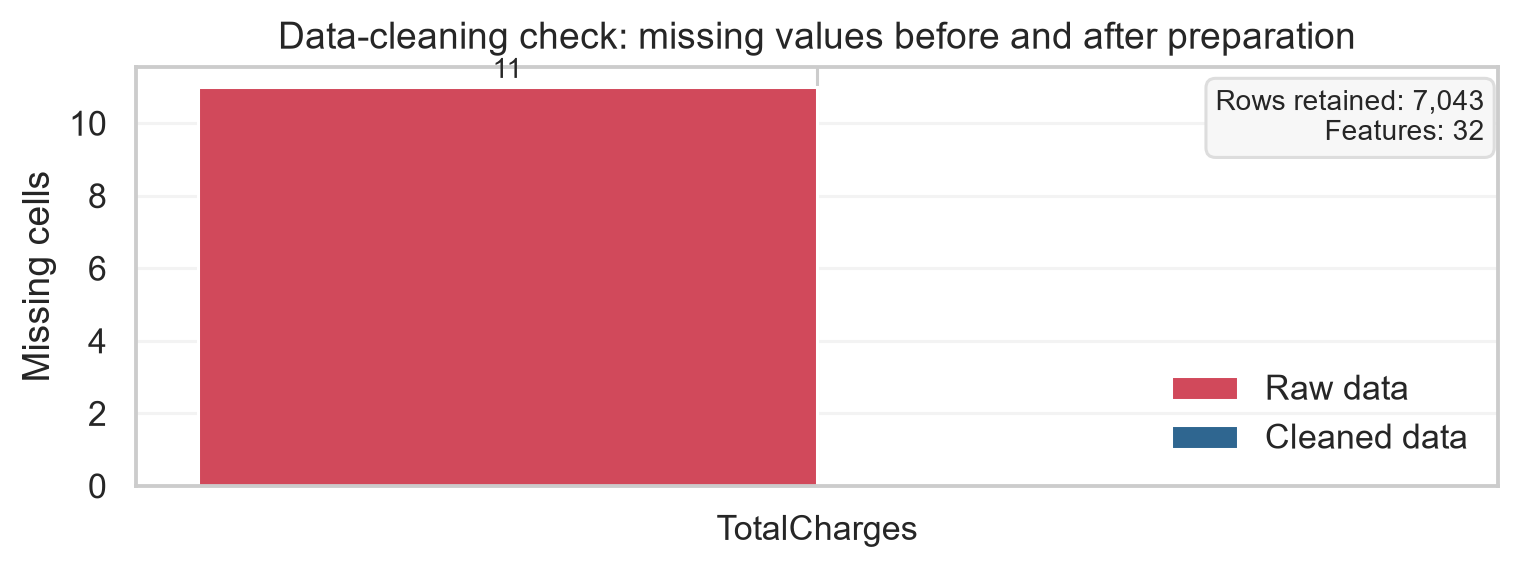
\includegraphics[width=0.72\textwidth]{data_quality.png}
\caption{Data-quality evidence generated from the raw and cleaned files. The 11 whitespace values in \texttt{TotalCharges} are resolved by numeric coercion and imputation.}
\label{fig:data-quality}
\end{figure}

\figpair{churn_balance.png}{Observed target balance.}{tenure_distribution.png}{Tenure distributions by observed outcome.}
\figpair{monthly_charges.png}{Monthly-charge distributions by outcome.}{numeric_correlation.png}{Correlation of core numeric variables.}

\section*{4. Modelling and evaluation protocol}
TCCP benchmarks five models: elastic-net logistic regression, RBF SVC, random forest, XGBoost, and a PyTorch multilayer perceptron. Hyperparameters are tuned only on the training partition using five-fold validation PR-AUC. The independent test set is used once for final reporting. This prevents test-set performance from silently becoming a model-selection criterion.

The primary selection metric is PR-AUC because churn is an imbalanced positive class and the operational team needs a useful ranking of likely churners. ROC-AUC measures broad ranking quality; accuracy and balanced accuracy are secondary threshold metrics; Brier score measures squared probability error. Calibration is assessed with quantile-binned predicted probabilities against observed churn rates.

\begin{table}[!ht]
\centering\scriptsize
\begin{tabular}{lccccc}
\toprule
\textbf{Model} & \textbf{Validation PR-AUC} & \textbf{Test ROC-AUC} & \textbf{Test PR-AUC} & \textbf{Accuracy} & \textbf{Balanced accuracy}\\
\midrule
SVC (RBF) & 0.670 $\pm$ 0.019 & 0.846 $\pm$ 0.011 & 0.667 $\pm$ 0.025 & 0.755 & 0.759\\
Logistic regression & 0.670 $\pm$ 0.016 & 0.848 $\pm$ 0.011 & 0.665 $\pm$ 0.025 & 0.760 & 0.763\\
Neural network (MLP) & 0.668 $\pm$ 0.016 & 0.846 $\pm$ 0.011 & 0.653 $\pm$ 0.026 & 0.779 & 0.757\\
XGBoost & 0.666 $\pm$ 0.021 & 0.844 $\pm$ 0.011 & 0.657 $\pm$ 0.025 & 0.774 & 0.753\\
Random forest & 0.665 $\pm$ 0.020 & 0.845 $\pm$ 0.011 & 0.655 $\pm$ 0.026 & 0.768 & 0.769\\
\bottomrule
\end{tabular}
\caption{Benchmark results on the independent test set. Uncertainty values are bootstrap standard deviations where available. The SVC is the TCCP champion by validation PR-AUC.}
\label{tab:benchmark}
\end{table}

\begin{figure}[!ht]
\centering
\includegraphics[width=0.86\textwidth]{model_metrics.png}
\caption{Model comparison across ranking and threshold metrics.}
\label{fig:metrics}
\end{figure}

\figpair{roc_pr_curves.png}{ROC and precision-recall curves from the test predictions.}{calibration_test.png}{Empirical calibration by probability decile.}

\section*{5. Explainability: from score to reason}
TCCP uses explanations as decision support, not as causal claims. SHAP values describe how the fitted model moves an individual prediction relative to a background sample. Positive SHAP values increase predicted churn output; negative values reduce it. Partial dependence shows the model's average response when one feature is varied while other rows are retained. These views answer different questions: SHAP explains local and global model behavior, while partial dependence summarizes an average response curve.

\begin{figure}[!ht]
\centering
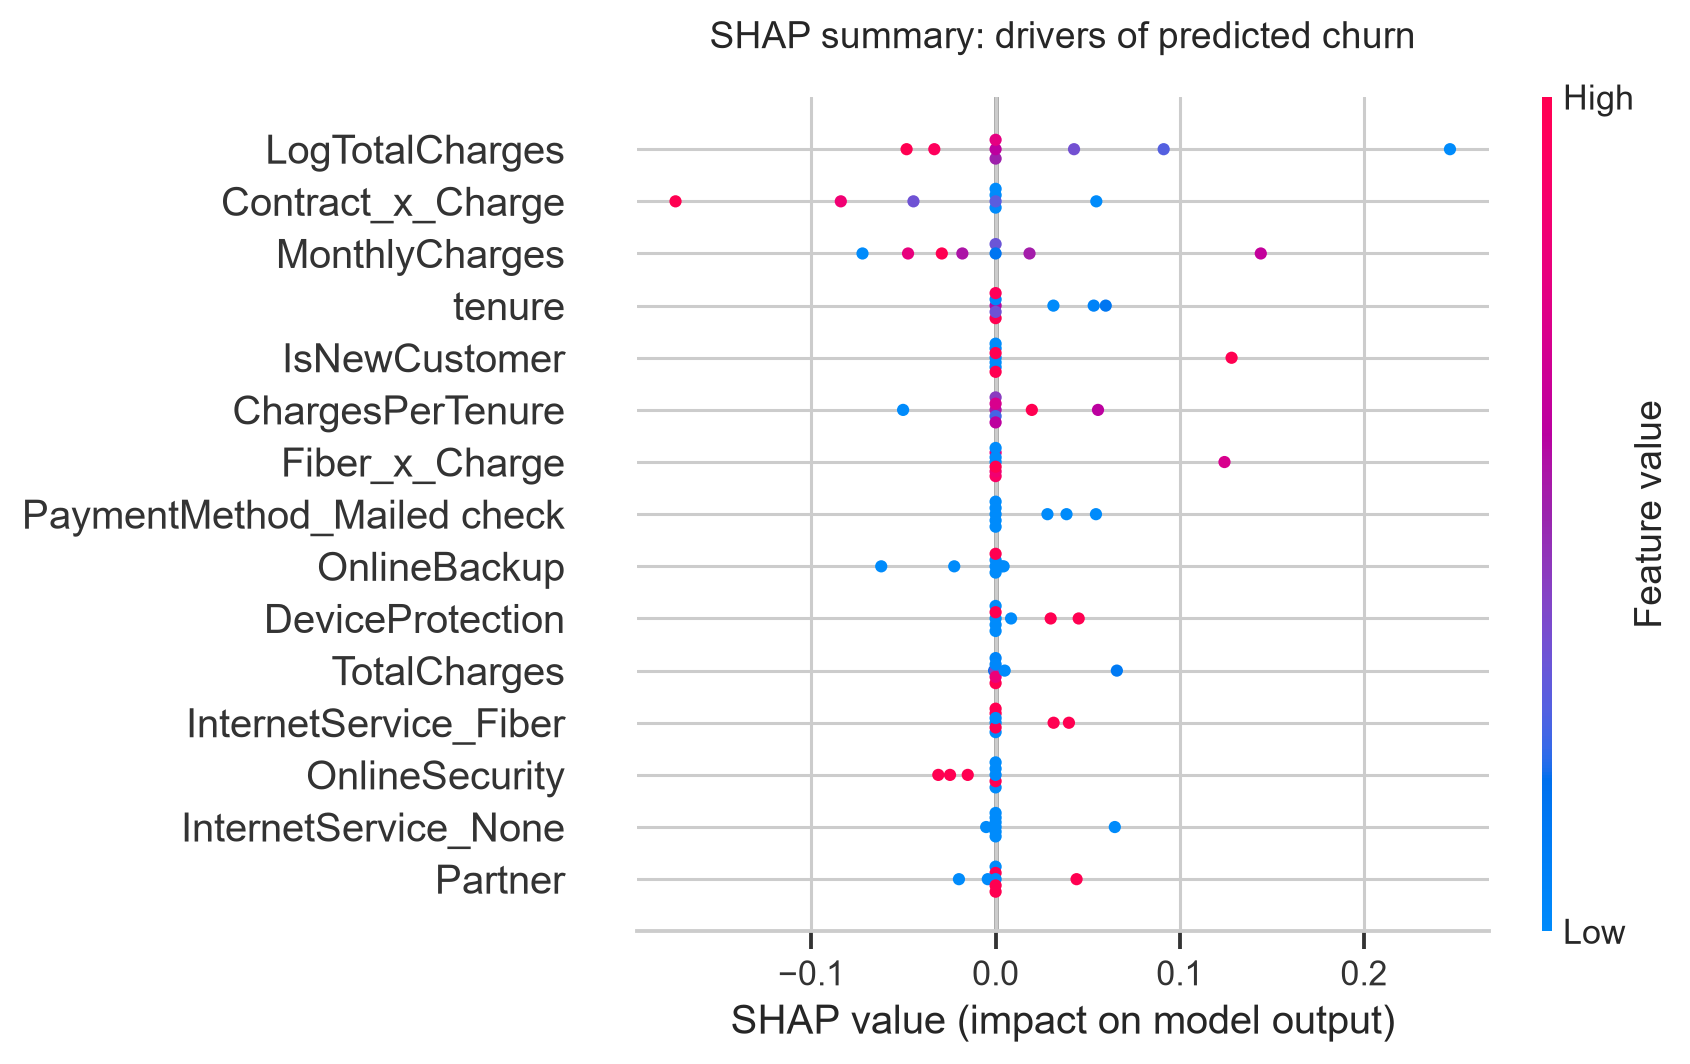
\includegraphics[width=0.83\textwidth]{shap_summary.png}
\caption{SHAP summary plot from real test-set rows. Feature importance and direction describe model behavior, not intervention causality.}
\label{fig:shap-summary}
\end{figure}

\begin{figure}[!ht]
\centering
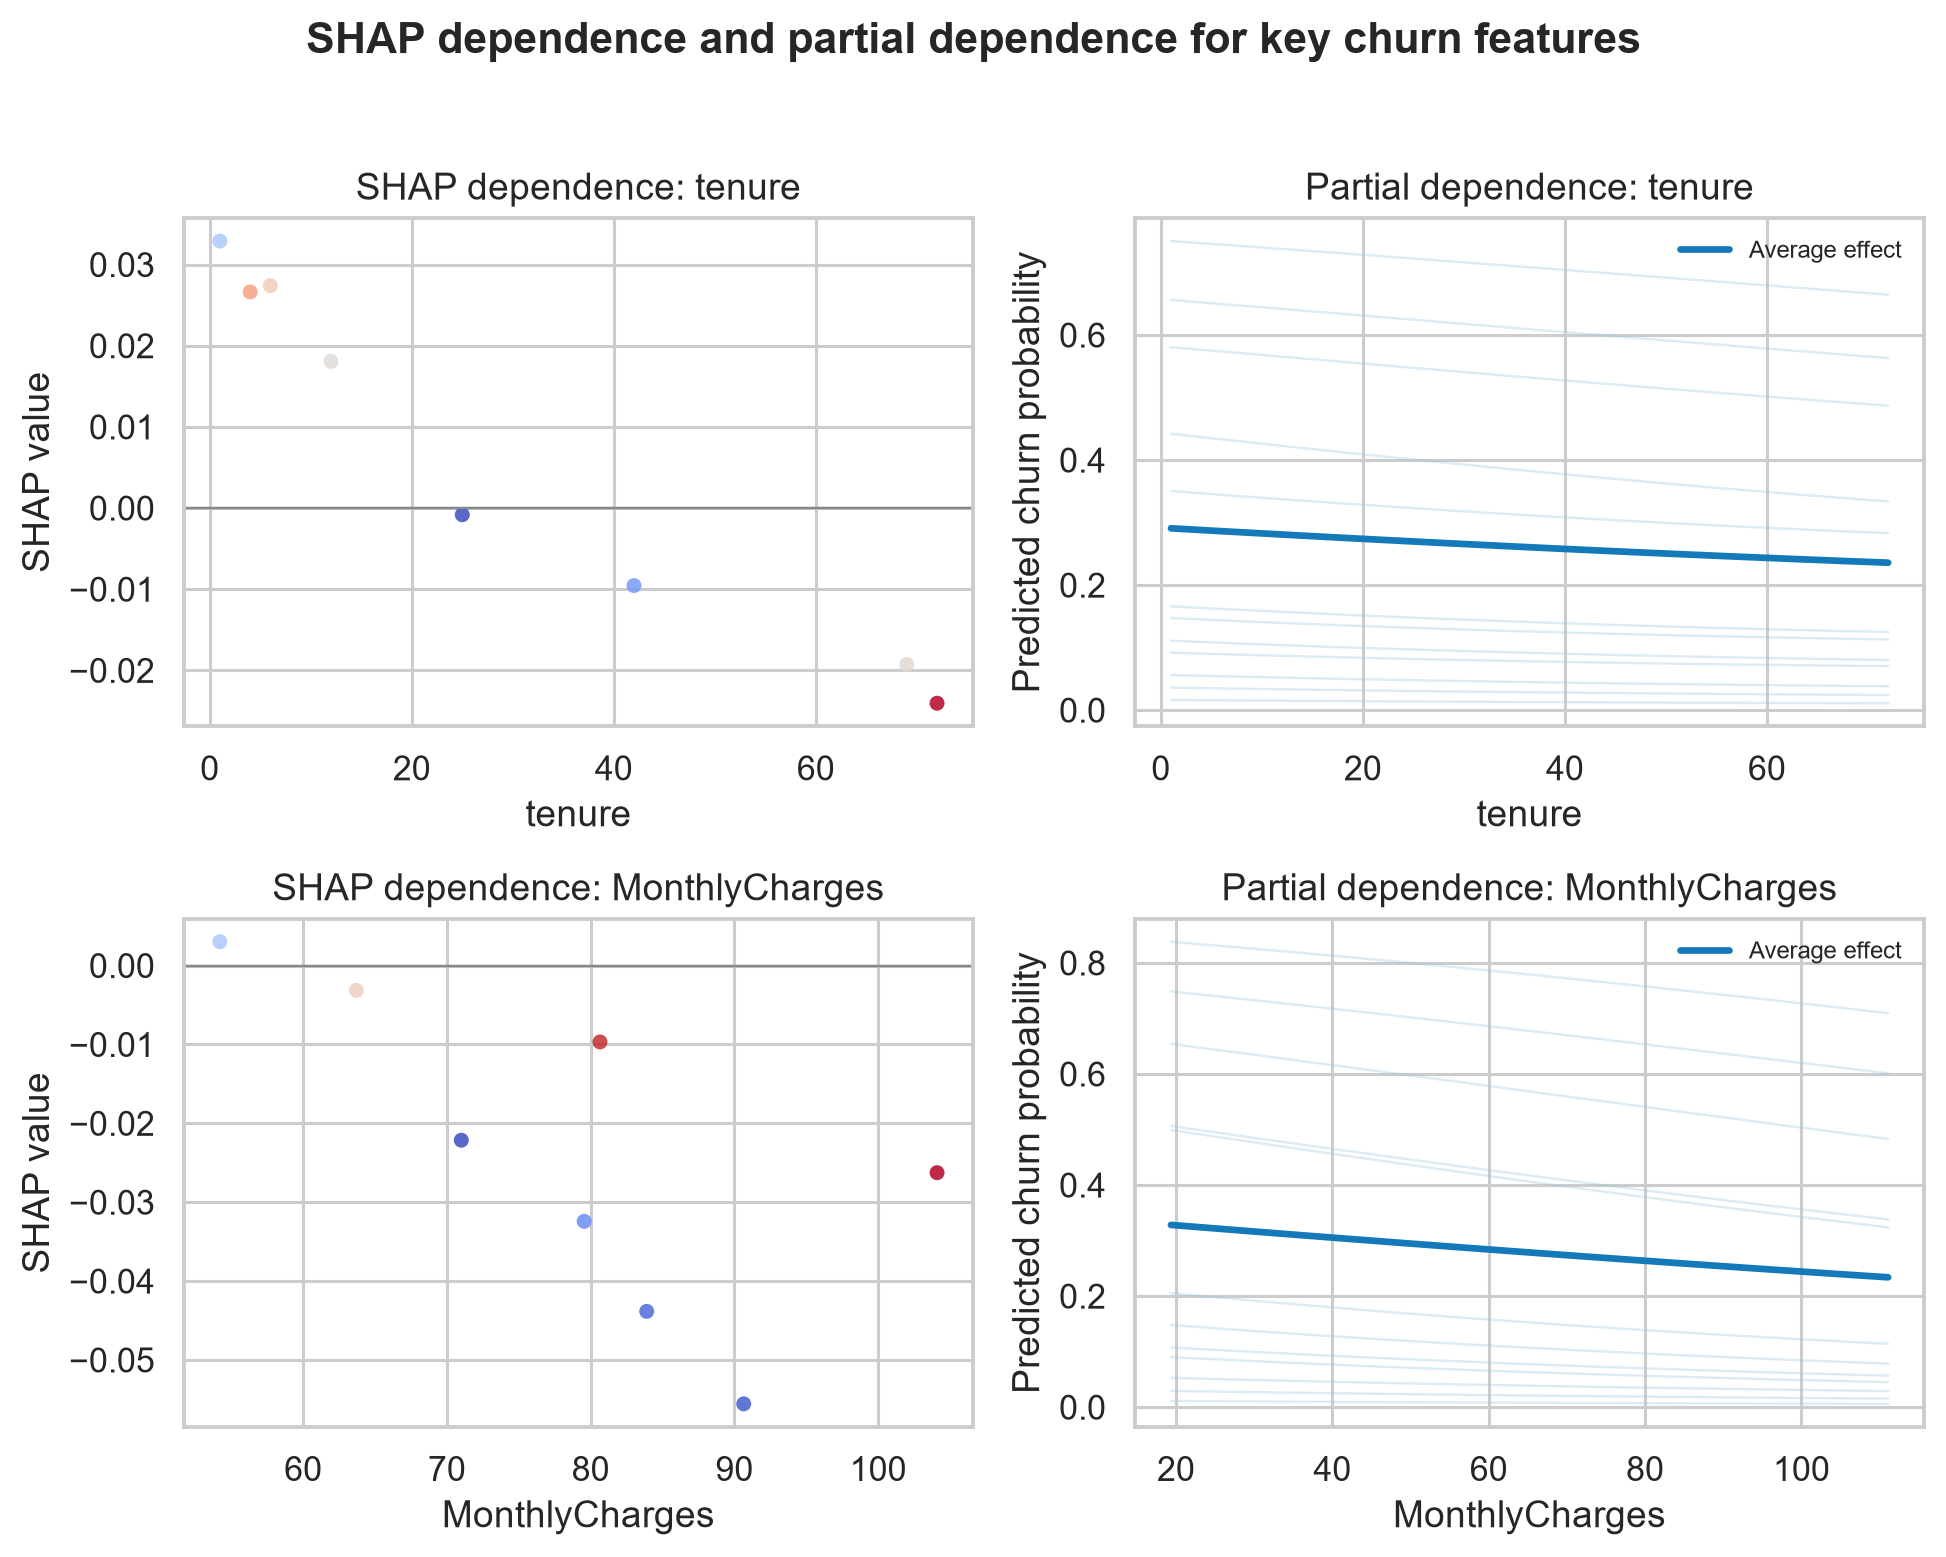
\includegraphics[width=0.94\textwidth]{shap_pdp_dependence.png}
\caption{SHAP dependence and partial-dependence plots for tenure and MonthlyCharges. The plots are generated from the trained SVC and real test-set data.}
\label{fig:shap-pdp}
\end{figure}

\begin{figure}[!ht]
\centering
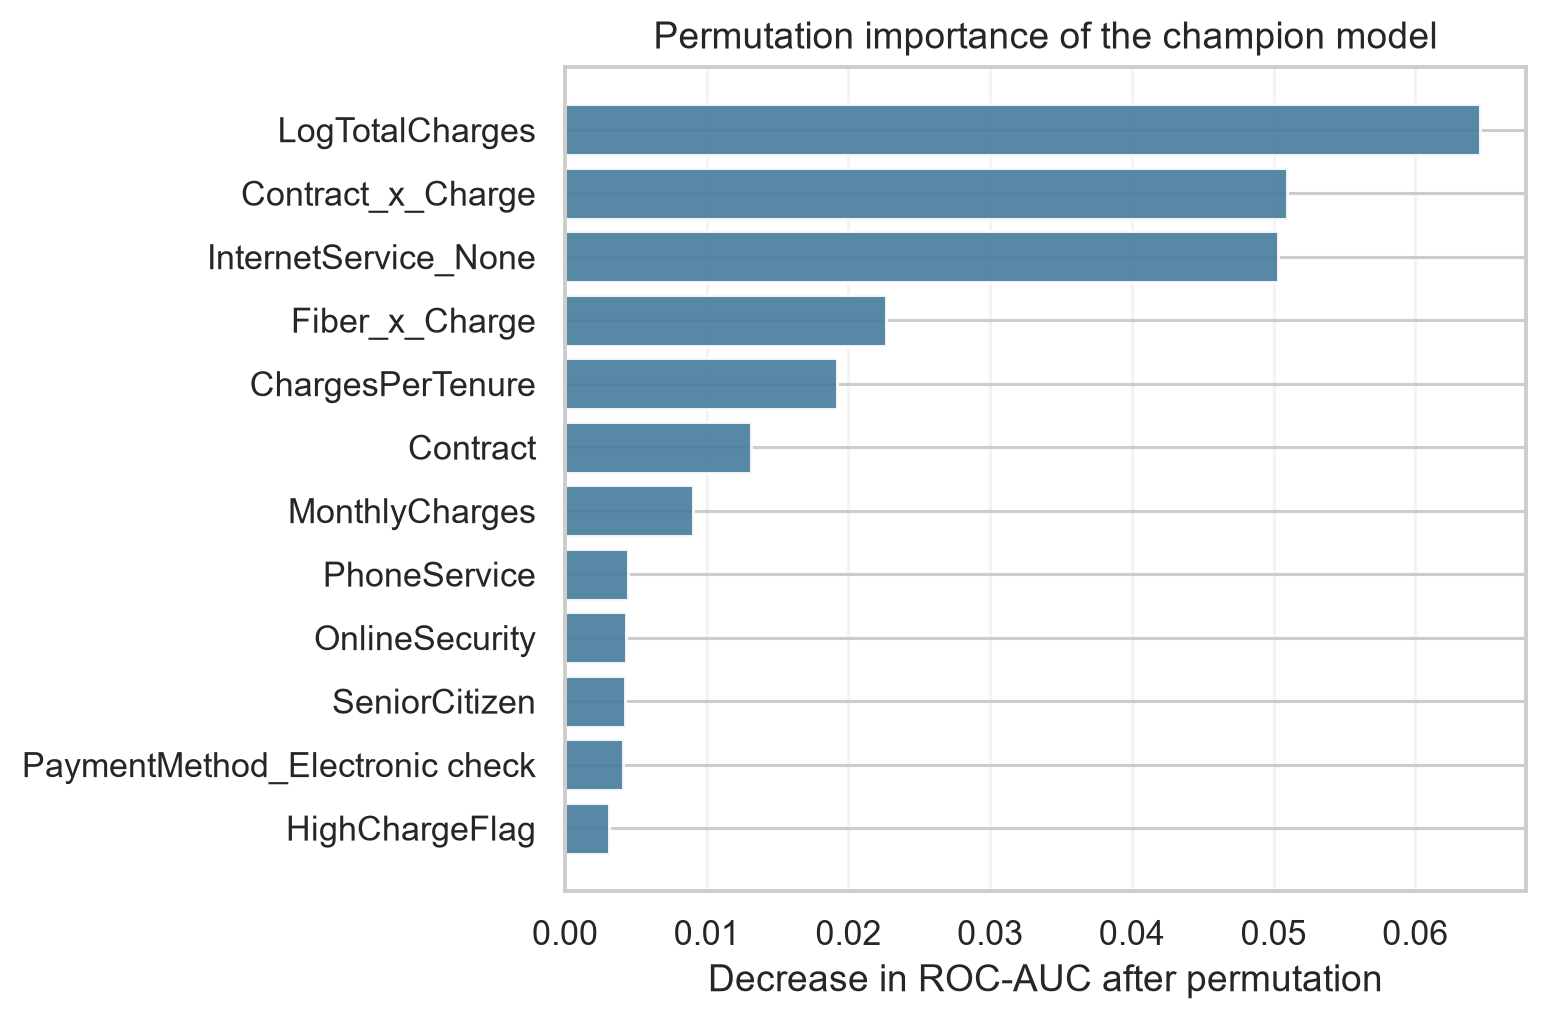
\includegraphics[width=0.82\textwidth]{permutation_importance.png}
\caption{Model-agnostic permutation importance measured as the decrease in test ROC-AUC after feature permutation.}
\label{fig:permutation}
\end{figure}

The explanations support actionable hypotheses. For example, tenure, contract-charge interactions, monthly charges, and service indicators can guide retention experiments. They do not prove that changing a contract or charge will cause a customer to stay; that question requires randomized intervention measurement.

\section*{6. Prediction-to-action policy}
The model output is a probability, not an automatic offer. TCCP applies an explicit policy: rank customers by predicted churn probability, apply a targeting threshold of 0.30 for the retention workflow, and select the highest-ranked customers until the budget is consumed. The conventional 0.50 classification threshold remains visible for comparison but is not assumed to be the economically optimal intervention threshold.

For the demonstration scenario, the save rate is $r=0.25$, customer value is $v=\$200$, and contact cost is $c=\$5$. The break-even probability implied by the simple utility expression is $c/(rv)=0.10$; the practical campaign threshold is stricter because contacts are ranked, capacity is limited, and the save-rate assumption is uncertain.

\begin{table}[!ht]
\centering\small
\begin{tabular}{lll}
\toprule
\textbf{Tier} & \textbf{Risk rule} & \textbf{Suggested action}\\
\midrule
Immediate intervention & $p\geq0.50$ & High-touch retention offer or priority call\\
Nurture sequence & $0.30\leq p<0.50$ & Targeted message, service review, or incentive test\\
Monitor & $p<0.30$ & Standard service and drift monitoring\\
\bottomrule
\end{tabular}
\caption{Demonstration action tiers. The tiers are policy choices and should be validated with intervention outcomes.}
\label{tab:tiers}
\end{table}

\begin{figure}[!ht]
\centering
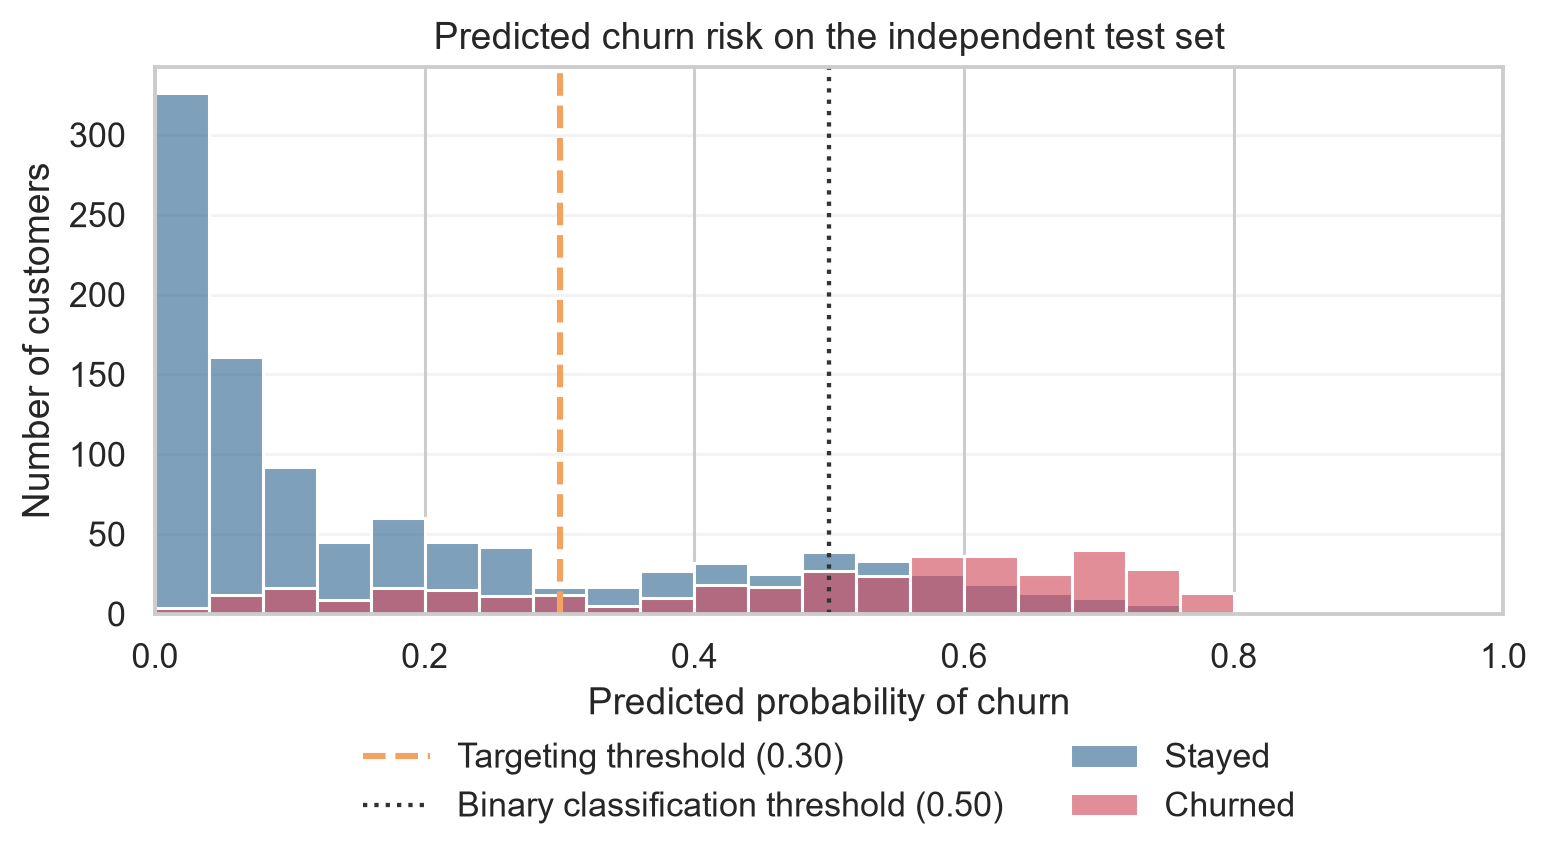
\includegraphics[width=0.93\textwidth]{prediction_risk.png}
\caption{Predicted churn-risk distribution on the independent test set, with targeting and binary-classification reference thresholds.}
\label{fig:risk}
\end{figure}

\begin{figure}[!ht]
\centering
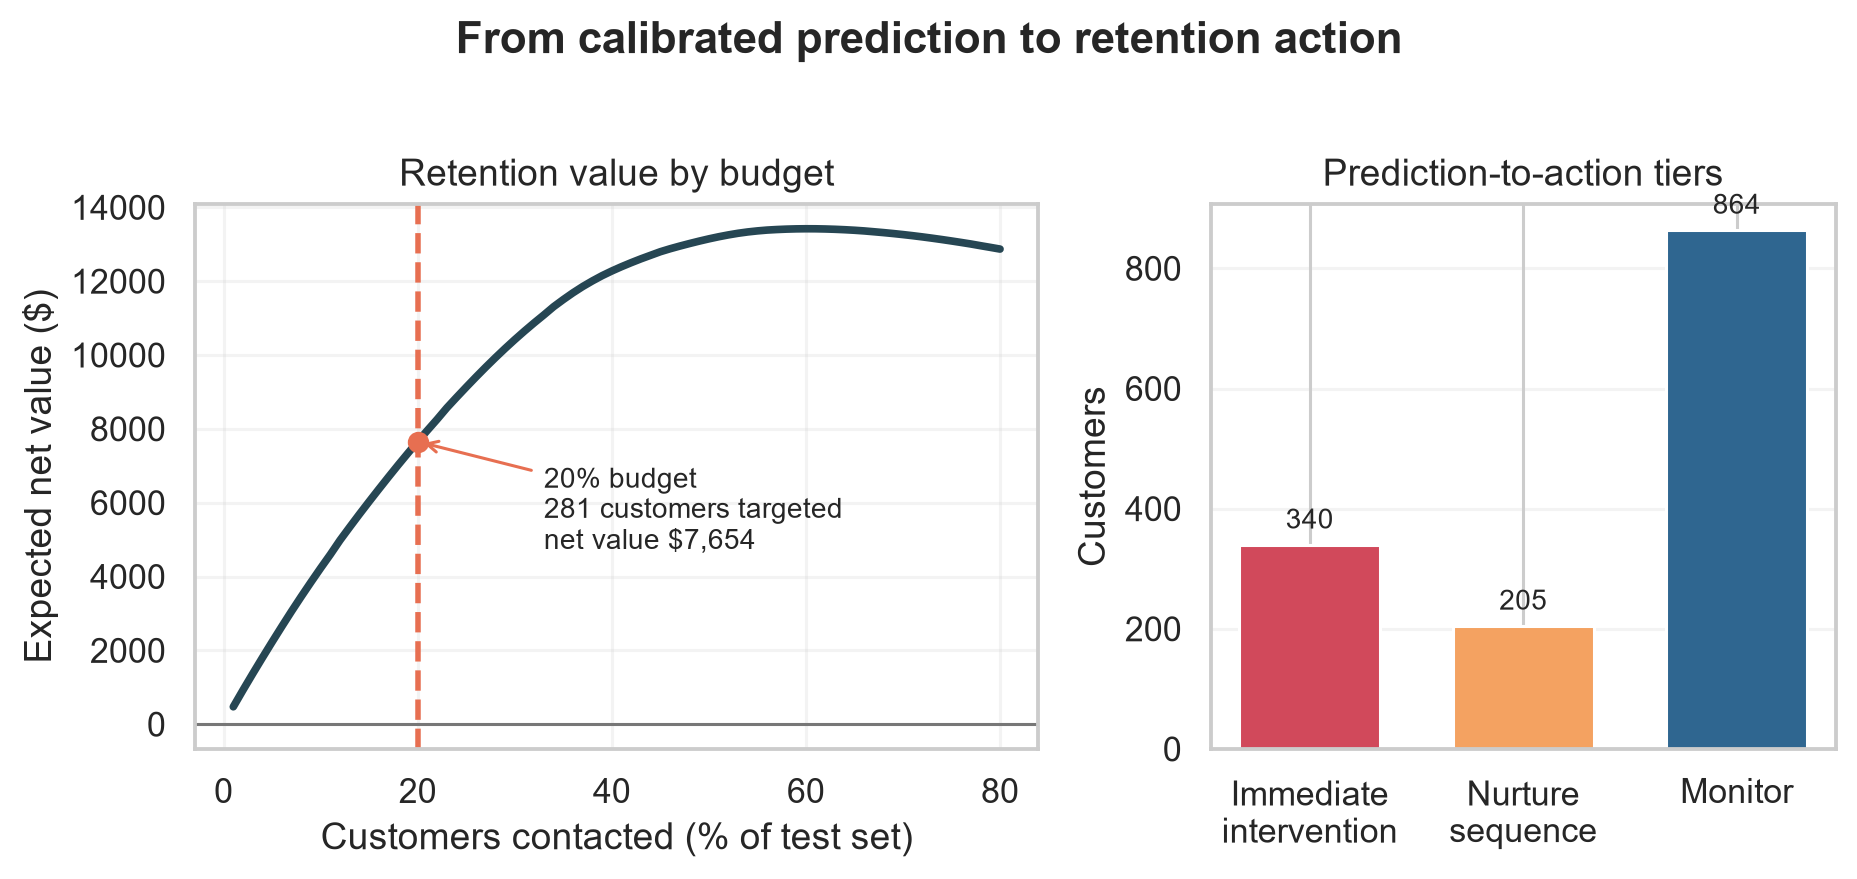
\includegraphics[width=0.94\textwidth]{retention_action.png}
\caption{Retention action graph: expected net value by contact budget and the resulting prediction-to-action tiers.}
\label{fig:action}
\end{figure}

At a 20\% contact budget, the test-set simulation targets 281 customers and estimates approximately \$7,654 in net value under the stated assumptions. This is a scenario estimate, not an observed causal return. Production use should replace the assumed save rate and value with measured treatment outcomes and confidence intervals.

\section*{7. Production and MLOps design}
The TCCP production path has four controls. First, the feature contract ensures that inference receives the same 32 engineered columns used during training. Second, the model artifact stores the fitted preprocessing and estimator together, avoiding inconsistent transformations between training and serving. Third, the model registry separates versions and stages; the local registry uses a production stage and the deployment design supports a champion alias. Fourth, operational interfaces expose both batch and online scoring.

The FastAPI service provides health and metadata endpoints and a bounded \texttt{/predict} request containing one to 10,000 records. Batch scoring processes input in chunks and appends \texttt{predicted\_churn\_probability} and \texttt{predicted\_churn}. The CI/CD workflow validates the repository and can run the Databricks job with controlled dependencies. MLflow records parameters, metrics, signatures, and the serialized model for lineage.

\begin{center}
\begin{tabular}{p{0.25\textwidth}p{0.61\textwidth}}
\toprule
\textbf{Control} & \textbf{TCCP implementation}\\
\midrule
Reproducibility & Seed 42, versioned code, feature metadata, benchmark CSV, serialized artifacts.\\
Data safety & Target and identifier removed before inference; unknown categories handled by the encoder.\\
Model governance & Registry name/stage, champion model metadata, model version, and health endpoint.\\
Deployment & Batch scoring CLI, FastAPI service, Docker image, GitHub Actions workflow.\\
Monitoring & Calibration drift, input-schema errors, score distribution, intervention outcomes, and model performance.\\
\bottomrule
\end{tabular}
\end{center}

\section*{8. Limitations, safeguards, and next steps}
The dataset is historical and does not establish future performance or causal treatment effects. The random holdout does not replace a time-based holdout when deployment dates are known. SHAP and partial dependence explain the fitted model but cannot establish that a feature causes churn. The retention simulation depends on assumed save rate, value, and cost; each should be estimated from experiments. Subgroup calibration and error rates should also be checked before operational use, particularly for customers who may be disproportionately affected by automated offers.

The next TCCP release should add four safeguards: a time-based validation set, calibration monitoring by cohort, randomized retention experiments, and an approval gate that prevents a model from becoming the production champion without passing data-quality and fairness checks. These controls convert a strong offline benchmark into a responsible decision system.

\section*{9. Conclusion}
TCCP solves the complete churn workflow rather than optimizing one isolated metric. It starts with a reproducible data contract, compares models under a leakage-safe protocol, selects and evaluates a calibrated champion, explains risk with SHAP and partial dependence, translates probabilities into a budget-aware action policy, and packages the result for governed serving. The central result is not simply an ROC-AUC value: it is a traceable path from a customer record to a defensible retention decision.

\newpage
\section*{Appendix A. Production feature schema}
The production artifact records the following 32-column feature contract. Identifiers and the target label are excluded before inference.

\small
\begin{longtable}{p{0.37\textwidth}p{0.53\textwidth}}
\caption{Production feature schema and interpretation.}\label{tab:features}\\
\toprule
\textbf{Feature} & \textbf{Interpretation}\\
\midrule
\endfirsthead
\toprule
\textbf{Feature} & \textbf{Interpretation}\\
\midrule
\endhead
\bottomrule
\endfoot
SeniorCitizen & Senior-citizen indicator.\\
Partner & Whether the customer has a partner.\\
Dependents & Whether the customer has dependents.\\
tenure & Months the customer has remained active.\\
PhoneService & Whether phone service is subscribed.\\
MultipleLines & Multiple-line phone-service category.\\
OnlineSecurity & Online-security service category.\\
OnlineBackup & Online-backup service category.\\
DeviceProtection & Device-protection service category.\\
TechSupport & Technical-support service category.\\
StreamingTV & Streaming-TV service category.\\
StreamingMovies & Streaming-movies service category.\\
Contract & Contract term category.\\
PaperlessBilling & Paperless-billing indicator.\\
MonthlyCharges & Recurring monthly charge.\\
TotalCharges & Total customer charge.\\
gender\_Male & One-hot encoded gender category.\\
InternetService\_Fiber & Fiber internet indicator.\\
InternetService\_None & No-internet-service indicator.\\
PaymentMethod\_Credit card (automatic) & Automatic credit-card payment indicator.\\
PaymentMethod\_Electronic check & Electronic-check payment indicator.\\
PaymentMethod\_Mailed check & Mailed-check payment indicator.\\
AutoPay & Automatic-payment feature.\\
NumServices & Count of subscribed services.\\
TenureBin & Discretized tenure group.\\
HighChargeFlag & Indicator for relatively high charges.\\
Contract\_x\_Charge & Contract-charge interaction.\\
Fiber\_x\_Charge & Fiber-charge interaction.\\
ChargesPerTenure & Charge normalized by tenure.\\
LogMonthlyCharges & Log-transformed monthly charge.\\
LogTotalCharges & Log-transformed total charge.\\
IsNewCustomer & New-customer indicator.\\
\end{longtable}

\section*{Appendix B. Reproducibility commands}
\begin{verbatim}
env\Scripts\python.exe src\decision_visuals.py
env\Scripts\python.exe -m src.batch_score \
  --input data/telco_clean_32col.csv \
  --output artifacts/scored_customers.csv
\end{verbatim}
The first command regenerates the Matplotlib/Seaborn/SHAP figures from the project artifacts. The second command demonstrates batch prediction through the production feature contract.

\end{document}
